\documentclass[aspectratio=169]{beamer}
\usetheme{Madrid}
\usecolortheme{default}
\usepackage{amsmath,amssymb,booktabs,graphicx}

\title{Multi-Exposure Modelling of Information Spread Through Social Media Reposting}
\author{Lavanya Kumar}
\institute{MATH 4090}
\date{Project Presentation}

\begin{document}

\begin{frame}
  \titlepage
\end{frame}

\begin{frame}{Presentation Roadmap}
  \begin{enumerate}
    \item Topic and background
    \item My model and assumptions
    \item Equilibria, Jacobian, and what they mean
    \item Simulation results and interpretation
    \item Remaining work for the final report
  \end{enumerate}
\end{frame}

\begin{frame}{Topic and Motivation}
  \textbf{Main question:} how does one post spread when people may need repeated exposures before reposting?

  \vspace{0.4em}
  Why this matters:
  \begin{itemize}
    \item On Instagram, people often see the same content multiple times.
    \item Some users repost quickly, some need reinforcement, and some lose interest.
    \item A simple one-step SIR-style model does not track repeated exposure.
  \end{itemize}

  \vspace{0.4em}
  \textbf{Goal:} build a simple ODE model that can show viral spread, moderate spread, and fizzle-out behaviour.
\end{frame}

\begin{frame}{Background and Existing Modelling}
  This project is related to three modelling ideas:
  \begin{itemize}
    \item \textbf{Rumor models:} Daley--Kendall and Maki--Thompson track spreaders and stiflers.
    \item \textbf{Threshold / complex contagion models:} repeated exposure can matter before adoption.
    \item \textbf{Network diffusion models:} social structure affects how cascades grow.
  \end{itemize}

  \vspace{0.5em}
  \textbf{What is new here?}
  \begin{itemize}
    \item I keep the model simple with ODEs.
    \item I explicitly track exposure classes $I_0, I_1, \dots, I_m$.
    \item This lets repeated views matter without building a full network model.
  \end{itemize}
\end{frame}

\begin{frame}{Compartments in Simple Terms}
  \begin{itemize}
    \item $I_0(t)$: users who have not yet been exposed
    \item $I_1(t)$: users exposed once, not yet sharing
    \item $I_2(t)$: users exposed twice, not yet sharing
    \item $\dots$
    \item $S(t)$: active sharers
    \item $R(t)$: saturated users who will not share further
  \end{itemize}

  \vspace{0.4em}
  Population is conserved:
  \[
  I_0 + I_1 + \cdots + I_m + S + R = N.
  \]

  \vspace{0.4em}
  \textbf{Important clarification from the meeting:}
  \begin{itemize}
    \item For the disease-free equilibrium, we set $I_0=N$ and all other classes equal to $0$.
    \item For simulations, I use a small initial seed of sharers, so typically $I_0(0)=N-S(0)$ and $S(0)>0$.
  \end{itemize}
\end{frame}

\begin{frame}{How Users Move Between Classes}
  Exposure rate:
  \[
  \lambda(t)=\frac{\beta S(t)}{N}.
  \]

  \begin{itemize}
    \item $\beta$: repost intensity or visibility
    \item If a user is in $I_i$, then on exposure:
    \begin{itemize}
      \item they share with probability $\rho_i$,
      \item they saturate with probability $\sigma_i$,
      \item otherwise they move to the next class.
    \end{itemize}
    \item Sharers leave $S$ at rate $\gamma$.
  \end{itemize}

  \vspace{0.4em}
  \textbf{Additional condition:}
  \[
  0 \le \rho_i,\sigma_i \le 1,
  \qquad
  \rho_i+\sigma_i \le 1.
  \]
  This ensures the remaining probability $1-\rho_i-\sigma_i$ is valid.
\end{frame}

\begin{frame}{Key Equations and the $I_0 \to I_1$ Step}
  \[
  \frac{dI_0}{dt}=-\lambda I_0
  \]
  Users leave $I_0$ when sharers expose them.

  \vspace{0.4em}
  \[
  \frac{dI_1}{dt}=(1-\rho_0-\sigma_0)\lambda I_0-\lambda I_1
  \]

  \textbf{Interpretation of $I_0 \to I_1$:}
  \begin{itemize}
    \item A user in $I_0$ gets exposed at rate $\lambda I_0$.
    \item If they do \emph{not} share and do \emph{not} saturate after that exposure, they move into $I_1$.
    \item So the inflow into $I_1$ is $(1-\rho_0-\sigma_0)\lambda I_0$.
  \end{itemize}

  \vspace{0.4em}
  This is the main reinforcement idea in the model.
\end{frame}

\begin{frame}{Variables and Parameters}
  \small
  \begin{tabular}{ll}
    \toprule
    Symbol & Meaning / where it is used \\
    \midrule
    $N$ & total population, conservation equation and $\lambda=\beta S/N$ \\
    $I_i(t)$ & users exposed exactly $i$ times and not yet sharing \\
    $S(t)$ & active sharers, drives new exposure \\
    $R(t)$ & saturated users, no longer share \\
    $\beta$ & repost intensity in $\lambda$ \\
    $\gamma$ & rate sharers stop sharing, appears in $dS/dt$ \\
    $\rho_i$ & probability of sharing from class $I_i$, appears in $dS/dt$ \\
    $\sigma_i$ & probability of saturation from class $I_i$, appears in $dR/dt$ \\
    \bottomrule
  \end{tabular}

  \vspace{0.5em}
  \normalsize
  \textbf{Professor comment addressed:} $\rho_i$ and $\sigma_i$ are now explicitly included and explained in the table.
\end{frame}

\begin{frame}{Equilibria}
  \textbf{1. Disease-free equilibrium}
  \[
  E_0=(I_0,I_1,I_2,S)=(N,0,0,0), \qquad R=0.
  \]
  Interpretation: nobody is sharing, so no new exposures happen.

  \vspace{0.6em}
  \textbf{2. Absorbing / burned-out equilibrium}
  \[
  E_\ast=(0,0,0,0), \qquad R=N.
  \]
  Interpretation: eventually everyone ends up saturated and the content dies out.

  \vspace{0.6em}
  \textbf{Why equilibria matter}
  \begin{itemize}
    \item They tell us the long-run resting states of the system.
    \item Then we study stability to ask: if we start near one equilibrium, do we stay near it or move away?
  \end{itemize}
\end{frame}

\begin{frame}{Jacobian and Local Stability}
  For $m=2$, linearizing around the disease-free equilibrium gives
  \[
  J(E_0)=
  \begin{pmatrix}
  0 & 0 & 0 & -\beta \\
  0 & 0 & 0 & (1-\rho_0-\sigma_0)\beta \\
  0 & 0 & 0 & 0 \\
  0 & 0 & 0 & \rho_0\beta-\gamma
  \end{pmatrix}.
  \]

  \begin{itemize}
    \item First, I identify the equilibrium.
    \item Then I compute the Jacobian there.
    \item Then I examine the eigenvalues.
  \end{itemize}

  \vspace{0.4em}
  Key eigenvalue:
  \[
  \lambda_S=\rho_0\beta-\gamma.
  \]

  \begin{itemize}
    \item If $\rho_0\beta-\gamma<0$, tiny sharing tends to die out initially.
    \item If $\rho_0\beta-\gamma>0$, tiny sharing can initially grow.
  \end{itemize}
\end{frame}

\begin{frame}{Why the Jacobian Is Not the Whole Story}
  The Jacobian at $E_0$ only captures \emph{local} behaviour near
  \[
  (I_0,I_1,I_2,S)=(N,0,0,0).
  \]

  \vspace{0.4em}
  In this model:
  \begin{itemize}
    \item several eigenvalues are zero,
    \item the exposure chain is frozen when $S=0$,
    \item secondary effects through $I_1$ and $I_2$ become important once spread has started.
  \end{itemize}

  \vspace{0.4em}
  So I also use:
  \[
  R_{\mathrm{eff}} \approx \frac{\beta}{\gamma}p_{\mathrm{share}}
  \]
  and simulations to understand the larger nonlinear dynamics.
\end{frame}

\begin{frame}{Simulation Setup}
  I use Python and \texttt{odeint} with:
  \begin{itemize}
    \item $m=2$, $N=1000$
    \item initial seed $S(0)=15$
    \item $I_0(0)=985$, $I_1(0)=I_2(0)=0$, $R(0)=0$
    \item three scenarios: viral, moderate, and fizzle
  \end{itemize}

  \vspace{0.4em}
  Peer-friendly interpretation:
  \begin{itemize}
    \item larger $\beta$ means content is seen more through sharing,
    \item larger $\gamma$ means sharers lose interest faster,
    \item larger $\rho_i$ means sharing is more likely,
    \item larger $\sigma_i$ means dropping out is more likely.
  \end{itemize}
\end{frame}

\begin{frame}{Main Numerical Results}
  \small
  \begin{tabular}{lccc}
    \toprule
    Scenario & Peak $S(t)$ & Time to peak & Final $R(120)$ \\
    \midrule
    Viral & 321.66 & 51.29 & 981.56 \\
    Moderate & 171.51 & 114.39 & 593.46 \\
    Fizzle & 15.00 & 0.00 & 15.41 \\
    \bottomrule
  \end{tabular}

  \vspace{0.6em}
  \normalsize
  \textbf{Discussion of results}
  \begin{itemize}
    \item Viral: large cascade and most users end in $R$.
    \item Moderate: spread happens, but more slowly and with a smaller peak.
    \item Fizzle: the initial sharers never create a real cascade.
  \end{itemize}

  \vspace{0.4em}
  This supports the idea that repeated exposure plus parameter choices can produce very different outcomes.
\end{frame}

\begin{frame}{Figure 1: Comparison Across Scenarios}
  \centering
  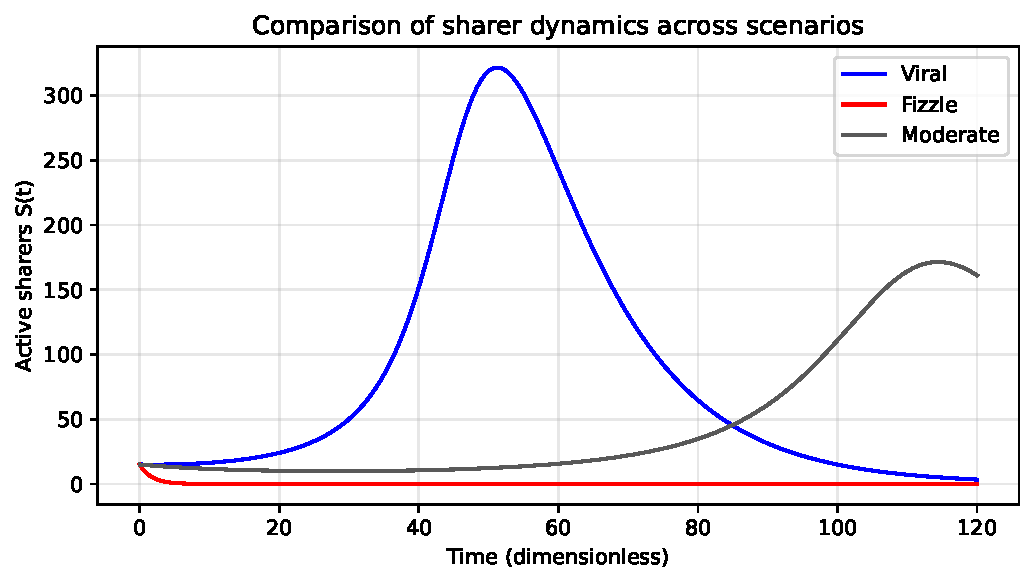
\includegraphics[width=0.78\textwidth]{fig_comparison.pdf}

  \vspace{0.3em}
  \footnotesize Figure caption: Active sharers $S(t)$ for viral, moderate, and fizzle scenarios.

  \vspace{0.4em}
  \normalsize
  Result: increasing effective spread creates a higher and earlier sharing peak; weak spread leaves the system near the initial seed.
\end{frame}

\begin{frame}{Figure 2: Exposure Classes in the Viral Case}
  \centering
  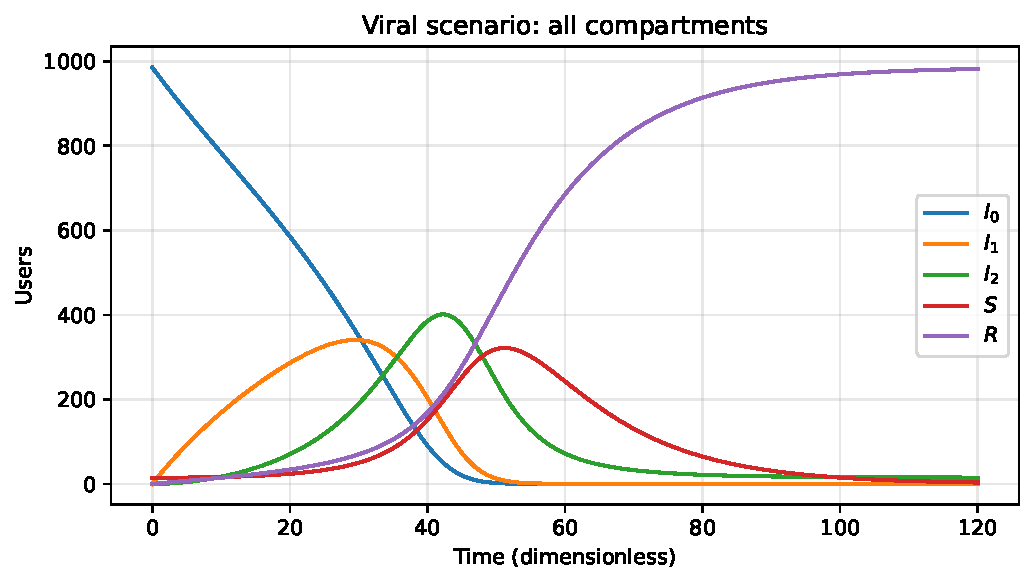
\includegraphics[width=0.78\textwidth]{fig_exposure_classes.pdf}

  \vspace{0.3em}
  \footnotesize Figure caption: Viral scenario showing $I_0$, $I_1$, $I_2$, $S$, and $R$ over time.

  \vspace{0.4em}
  \normalsize
  Result: users move out of $I_0$, pass through higher exposure classes, then either join $S$ or end in $R$.
\end{frame}

\begin{frame}{Figure 3: What $\rho$, $\sigma$, and $\gamma$ Do}
  \begin{itemize}
    \item $\rho_i$ controls how likely a user is to share after exposure level $i$.
    \item $\sigma_i$ controls how likely a user is to stop without sharing after exposure level $i$.
    \item $\gamma$ controls how quickly current sharers stop being active.
  \end{itemize}

  \vspace{0.4em}
  \centering
  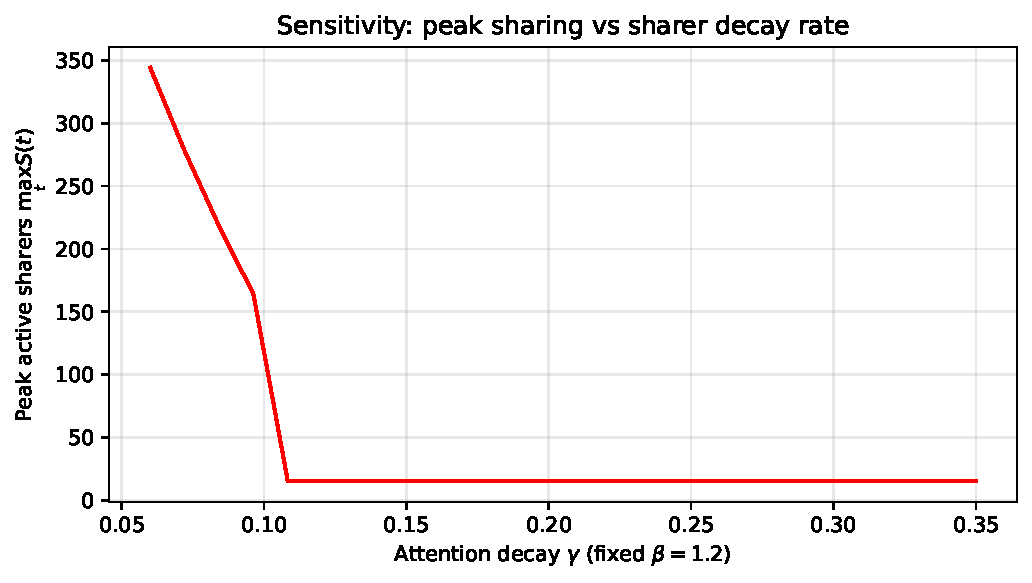
\includegraphics[width=0.72\textwidth]{fig_sensitivity_gamma.pdf}

  \vspace{0.3em}
  \footnotesize Figure caption: Peak active sharers as $\gamma$ changes, with other parameters fixed.

  \vspace{0.4em}
  \normalsize
  Result: when $\gamma$ increases, sharers disappear faster, so the peak becomes much smaller.
\end{frame}

\begin{frame}{What Still Needs to Be Completed}
  To finish the final report, I still need to:
  \begin{itemize}
    \item polish the equilibrium and stability discussion,
    \item make the Jacobian explanation more complete and cleaner,
    \item expand sensitivity analysis for $\gamma$, $\rho_i$, and $\sigma_i$,
    \item improve figure captions and figure-based discussion,
    \item tighten the connection between mathematical results and social-media interpretation.
  \end{itemize}

  \vspace{0.5em}
  \textbf{Current status:} the model, simulations, and main conclusions are already in place.
\end{frame}

\begin{frame}{Takeaway and Q\&A}
  \textbf{Main takeaway:}
  \begin{itemize}
    \item repeated exposure matters,
    \item a simple multi-exposure ODE model can capture viral, moderate, and fizzle outcomes,
    \item the balance among $\beta$, $\gamma$, $\rho_i$, and $\sigma_i$ determines whether a post grows or dies out.
  \end{itemize}

  \vspace{0.8em}
  \textbf{Possible audience questions to prepare for}
  \begin{itemize}
    \item Why not use a network model instead of homogeneous mixing?
    \item Why is $I_0=N$ at equilibrium but $I_0(0)=985$ in simulations?
    \item What do $\rho_i$ and $\sigma_i$ mean in real social-media terms?
    \item What is the limitation of using the Jacobian only at $E_0$?
  \end{itemize}
\end{frame}

\end{document}
